\documentclass[border=8pt]{standalone}
\usepackage{pgfplots}
\pgfplotsset{compat=1.18}
\begin{document}
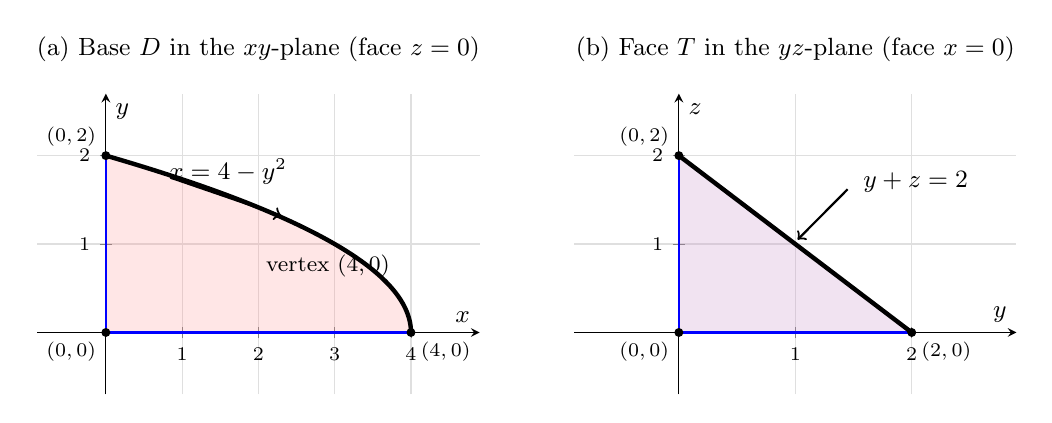
\begin{tikzpicture}

% ---------- (a) base region D in the xy-plane ----------
\begin{axis}[
    name=axA, width=7.2cm, height=5.4cm, at={(0,0)}, anchor=south west,
    xlabel={$x$}, ylabel={$y$},
    xmin=-0.9, xmax=4.9, ymin=-0.7, ymax=2.7,
    axis lines=middle,
    xtick={0,1,2,3,4}, ytick={0,1,2},
    ticklabel style={font=\scriptsize}, label style={font=\small},
    title={(a) Base $D$ in the $xy$-plane (face $z=0$)},
    title style={font=\small, yshift=2pt},
    grid=major, grid style={gray!25},
    samples=120, domain=0:4,
]
\addplot[fill=red!45, opacity=0.22, draw=none, smooth] (x, {sqrt(4-x)}) \closedcycle;
\addplot[ultra thick, black, smooth, domain=0:2] ({4-x^2}, {x});
\addplot[thick, blue] coordinates {(0,0) (0,2)};
\addplot[thick, blue] coordinates {(0,0) (4,0)};
\addplot[only marks, mark=*, mark size=1.4pt, black] coordinates {(0,0) (4,0) (0,2)};
\node[font=\scriptsize, anchor=north east] at (axis cs:0,0) {$(0,0)$};
\node[font=\scriptsize, anchor=north west] at (axis cs:4,0) {$(4,0)$};
\node[font=\scriptsize, anchor=south east] at (axis cs:0,2) {$(0,2)$};
\draw[->, thick] (axis cs:0.85,1.75) -- (axis cs:2.3,1.32);
\node[font=\small, anchor=west] at (axis cs:0.7,1.82) {$x=4-y^2$};
\node[font=\footnotesize, anchor=east] at (axis cs:3.85,0.75) {vertex $(4,0)$};
\end{axis}

% ---------- (b) face T in the yz-plane ----------
\begin{axis}[
    width=7.2cm, height=5.4cm, at={(axA.south east)}, anchor=south west, xshift=1.2cm,
    xlabel={$y$}, ylabel={$z$},
    xmin=-0.9, xmax=2.9, ymin=-0.7, ymax=2.7,
    axis lines=middle,
    xtick={0,1,2}, ytick={0,1,2},
    ticklabel style={font=\scriptsize}, label style={font=\small},
    title={(b) Face $T$ in the $yz$-plane (face $x=0$)},
    title style={font=\small, yshift=2pt},
    grid=major, grid style={gray!25},
]
\addplot[fill=violet!45, opacity=0.24, draw=none] coordinates {(0,0) (2,0) (0,2)} \closedcycle;
\addplot[thick, blue] coordinates {(0,0) (2,0)};
\addplot[thick, blue] coordinates {(0,0) (0,2)};
\addplot[ultra thick, black] coordinates {(0,2) (2,0)};
\addplot[only marks, mark=*, mark size=1.4pt, black] coordinates {(0,0) (2,0) (0,2)};
\node[font=\scriptsize, anchor=north east] at (axis cs:0,0) {$(0,0)$};
\node[font=\scriptsize, anchor=north west] at (axis cs:2,0) {$(2,0)$};
\node[font=\scriptsize, anchor=south east] at (axis cs:0,2) {$(0,2)$};
\draw[->, thick] (axis cs:1.45,1.62) -- (axis cs:1.02,1.05);
\node[font=\small, anchor=west] at (axis cs:1.5,1.70) {$y+z=2$};
\end{axis}

\end{tikzpicture}
\end{document}